\documentclass[]{article}
\usepackage[utf8]{inputenc}
\usepackage{hyperref}
\usepackage{listings}
\usepackage{epigraph}
\usepackage{fontspec}
\usepackage[toc,title]{appendix}

% Itemize with custom spacing
\newenvironment{myitemize}
{ \begin{itemize}
    \setlength{\itemsep}{0pt}
    \setlength{\parskip}{0pt}
    \setlength{\parsep}{0pt}     }
{ \end{itemize}                  }

%opening
\title{Tsukiji}
\author{Michael The \and Hugo Reinbergen}

\begin{document}

\maketitle

\section*{Related Work}
\begin{tabular}{|c|c|}
 \hline
 Document & Contents  \\
 \hline
 \url{http://tinyurl.com/ojjeqcc} & Online Marketplace \\
 \url{https://tinyurl.com/lrqbb2c} & Reputation \\
 \url{https://tinyurl.com/n3v5jsy} & Dispersy \\
 \url{https://bitcoin.org/bitcoin.pdf} & Bitcoin \\
 \url{http://www.weidai.com/bmoney.txt} & b-money \\
 Mailtje van Pouwelse & Credit Based P2P \\
 Book: Computer Networks & DHT, P2P \\
 \hline
\end{tabular}


\section{Preface}
This report describes the development process of creating a proof of concept for a decentral market, named Tsukiji. 
This proof of concept is created as part of the Bachelor Project course of the Computer Science program of Delft University of Technology.

We would like to thank Johan Pouwelse for giving us the opportunity to work on this project and provide guidance on how to attack the issue of decentralisation.
We also want to thank Raynor Vliegendhart for assisting us while developing the Bachelor Project report.
Finally, we want to give our thanks to Martha Larson and Felienne Hermans for supervising the project.

\begin{flushright}
Michael The \\
Hugo Reinbergen
\end{flushright}

\tableofcontents

\section{Summary} 
%problem description
File-sharing has become incredibly popular in recent years. 
Especially with the wide-spread adaption of BitTorrent. 
The big problem that peer-to-peer sharing brings is that the files need to be actively uploaded by users of the network.
To force users to upload actively rather than simply reap the benefits without work, small invite-based private groups are formed that only allow users that upload a certain amount of data, respectively to what they download.
In return, those groups can promise reliable download speed, since everyone is uploading frequently.
Due to various reasons, people cannot upload data, but still want to make use of the private groups.

To allow them to still participate, this project creates a marketplace to trade points for real money.
While many online marketplaces exist, they usually have one thing in common: a central point of authority.
Our solution is completely decentralised and is capable of scaling to 1000s of users.\\
\\
%research
Research showed that current implementations of this idea are scarce.
A couple of other proofs of concept have been published but never a true application that has not been shut down.
Since the project is in assignment of the group responsible for the creation of Tribler, this project follows their example in programming languages and libraries, such as Python and Twisted.\\
\\
%process
The development happened in sprints of around 1 week, focusing on one or two specific features.
After every development cycle, a meeting with the product owner showed what had to be created next and whether the current implementation was up to expectation.\\
\\
%implementation
The result is a light-weight terminal-based python application called Tsukiji.
The peers communicate by sending messages according to the gossip protocol and using the Twisted library.
Peers agreeing on a certain price can initiate a trade of which the financial transaction is made via PayPal.
With this, a fully decentralised market with a trustworthy payment system is created allowing users to make trades without the risk of their trading platform being shut down.
\section{Introduction}
\epigraph{The Internet is becoming the town square for the global village of tomorrow.}{Bill Gates}

The appearance of online marketplaces in the late 90s marked the beginning of a new era for consumers.
The connection between supplier and consumer is closer than ever.
Even trading between individuals has become commonplace.
Sites like ebay, Amazon and Alibaba all provide consumer-to-consumer, business-to-consumer and even business-to-business services.
Compared to traditional shopping, these platforms are easier to use, cost less time, have a wider range of products available and are better at matching buyer and seller.

Another example of such a marketplace is currency exchange platforms.
In recent years, Bitcoin has become of great interest to traders.
With the rise of interest in Bitcoin, the rise of Bitcoin exchange markets comes naturally.
The most famous of Bitcoin exchanges is the now defunct Mt.Gox.
Mt.Gox was plagued by problems early on that eventually led to its bankruptcy \cite{gox}.
With its downfall, it took a large amount of funds with it.
The trust users have put into the institution was violated.

% Third example: stock market?

Similar stories exist all over the place. Hacking attempts, government shutdowns, or simply incompetent companies.
These are all common among marketplaces of all kinds.
In this report we present \textit{tsukiji}, a decentralized marketplace.
This proof-of-concept marketplace has no central server bottleneck, no central point of trust, full self-organisation, and unbounded scalability.

%Torrents
Motivation and inspiration for creating Tsukiji originally came from Bittorrent communities.
The sharing of files has become more and more popular over the years.
Napster, Kazaa and LimeWire no longer exist, but one protocol has survived: BitTorrent.
BitTorrent is a peer-to-peer file sharing protocol.
Instead of downloading from a central server, each peer downloads from and uploads to other peers.
It offered a solution to the bottleneck of existing programs and protocols.

With more and more people using BitTorrent, the amount of people downloading files naturally increases.
Ideally, every peer should upload at least as much as they download.\cite{bittorrent}
Sadly, this does not happen in reality.
The amount of users only downloading and not uploading is significantly higher than people uploading at least as much as they download.
There is no incentive for an individual to upload, but with few peers who upload the download speed is significantly hampered.
To solve this issue, uploaders decided to work together in separate, private groups that only allow people with a good upload/download ratio.

This seems like a good solution to motivate peers to actively upload, but a couple of issues occur.\cite{bartercast}
With peers motivated to upload, a certain oversupply of uploading rises.
A peer with a low speed connection, has a hard time competing with many high-speed connections within the group.
This peer now loses reputation because of competition, even though they are putting in the effort to upload.

Unpopular files form another issue.
If someone downloads a large file and wants to upload it to increase his reputation, it is possible that there is not anyone that is interested in downloading that file.
This gives the peer a large deficit in his reputation that he cannot solve by uploading his unpopular taste.

Torrenting may also come with legal issues.
In some countries, such as Switzerland\cite{switzerland}, it is illegal to upload files, whereas downloading is allowed.
Citizens of such countries would like the high speed download of private communities, but cannot participate since they are legally not allowed to share whatever they have downloaded.

To solve these issues, peers need a way te obtain reputation in a way other than uploading.
We propose that users can trade reputation points for currency.
Reputation is still gained by uploading.
Peers can create offers on a marketplace to buy or sell reputation points.
This will give peers the incentive to upload data to the swarm.
At the same time, it will still be possible for peers to have access to the community by spending money and buying into a community.
This will lead to a more accessible and scalable community than traditional private torrent communities.

Keeping in line with BitTorrent's philosophy, Tsukiji will be fully decentralised and peer-to-peer.
With asynchronous cryptography, users will be able to keep their real identity hidden, while still being able to make trades with their network-alias.
Certain users will attempt to upload as much as possible to sell large amounts of reputation, keeping the network attractive with many uploaders.
With no central authority, the market is completely free to decide on a price for their reputation.
There is no added value of intermediaries since peers can directly sell to each other, keeping the price as low as possible.

% Conclusion?

% Insert description of each chapter, e.g. "In chapter 5 we will talk about wooly elephants."
\section{Problem definition}
%Torrents
Over the past years the sharing of files has become more and more popular. 
With this, many ways to share files have risen and fallen.
Napster, Kazaa and LimeWire no longer exist, but there is one protocol that has survived many attempts of large companies, BitTorrent.
Released in 2001, BitTorrent offered a solution to the bottleneck of the existing websites.
It did not contain a central server that contained data or a single website that offered links to data for peer to peer sharing.
In the worst case, a large website containing links to trackers of files get taken down, but those can easily be available on a different website. \\
\\
With more and more people starting to change to BitTorrent, the amount of people downloading a certain file increases.
This would not be a problem if every peer uploads an equal amount of data to what he downloads.
Sadly this does not happen.
The amount of users only downloading and not uploading is significantly higher than people uploading at least as much as they download.
This property is held with an increasing number of users, which leads to a bigger and bigger gap between uploaded and downloaded data.
To solve this issue, uploaders decided to work together in separate, private groups that only allow people that upload a certain percentage of their download.\\
\\
On the surface, this seems to be a good solution to motivate peers to upload actively, but it brings a couple of issues.
With peers motivated to upload, a certain oversupply of uploading rises.
A peer with a low speed connection, has a hard time competing with many high-speed connections within the group. The peer now loses reputation because of this competition even though the it is putting in effort to upload.

Another issue is unpopular files. 
If someone downloads a large file and wants to upload it to increase his reputation, it is possible that there are no users interested in downloading that file. 
This gives the peer a large deficit in his reputation that he cannot solve by uploading his unpopular taste.

Then there is also a legal problem that comes with torrenting. Some countries have banned the upload of files while allowing the download of files.
Citizens of such countries would like the high speed download of private communities but cannot participate since they are legally not allowed to share whatever they have downloaded.\\
\\
To solve these issues, peers need a way te receive reputation in a different way than uploading. We propose that users can receive reputation points in exchange for bitcoins. 
They can create incentive for a different user to seed more than would be necessary for that user, by offering money.
The peers can then create offers on a marketplace to buy and sell reputation points.
This way there is more of a reason to upload data to the swarm, but it will still be possible for peers to have access to the community buy spending money to reward other people effort, which will lead to a more accessible and scalable community than traditional private torrent communities.

To keep in line with the philosophy of BitTorrent, this system will be fully decentralised and peer to peer.
With secure cryptography, the users will be able to keep their real identity hidden, while still being able to make trades with their network-alias. 
In the same style as BitCoin, certain users will attempt to upload as much as they can just so they can sell large amounts of reputation, keeping the network attractive with very high download speeds.
With no central authority, the market is completely free to decide on a price for their reputation. There is essentially no added value of intermediaries since peers can directly sell to each other, keeping the price as low as possible.


\section{Requirements}

The goal of this project is to create a decentralised marketplace.
The basics of a marketplace should work, so users have to be able to trade (virtual) commodities.
The system should be decentralised.
It should scale to thousands of users.
A nice user interface is not a priority, so only command line input is required.

Spoofing of message would of course be a big problem in a trading network.
However, since this is a solved problem, the focus of the project should be on other areas.

It would be nice to ensure the privacy of the users.

In order to achieve this, strong encryption of messages is required.
Further thought is also necessary on what information is exposed.
It would be nice to have a network resistant against hostile takeover.
Having a decentralised system plays a big role in this.
However, other attack vectors could also be possible.
Finally, it would be nice to trade real, verified commodities.
Before we can do this however, the requirements listed above should be satisfied first.


The requirements are summarized in this MoSCoW list: \\

\begin{myitemize}
\item Must
\begin{myitemize}
	\item Place an ask/bid
	\item Trade an ask/bid
    \item Find each other (peer discovery)
    \item Decentralised
    \item Scalable to 1000s of users
    \item Command line input
\end{myitemize}
\item Should
\begin{myitemize}
	\item Anti-spoofing
\end{myitemize}
\item Could
\begin{myitemize}
	\item Nice User Interface
\end{myitemize}
\item Would
\begin{myitemize}
	\item Privacy
	\item Protection against attacks
	\item Trade real commodities (like Bitcoins)
\end{myitemize}
\end{myitemize}

\section{Implementation}
The development of Tsukiji followed aspects of the Scrum methodology. The weeks were divided into sprints. Each sprint lasted around a week. 
At the end of each sprint, the product owner is given a demo te discuss what should be developed in the next sprint.

\subsection{Sprint 1: Sockets, broadcasting and protocol definition}
In the first sprint, an early version of tsukiji was implemented. The goal of the first sprint was to create a local simulation of the decentral market using socket connections. Messages between peers are spread via broadcasting. A basic version of the message protocol is defined. Problems encountered during this sprint are also discussed: broken pipes with disconnected sockets, identifiers, and cancel messages.

\subsubsection{Broadcasting}
The peers have to be able to communicate with each other by passing messages.
The options considered for this were approaching a subset and relaying the information of your subset to other subsets and broadcasting your information to the entire network.
The issue that arose with the subset approach was that in a competitive market, someone that is selling an item is not easily motivated to advertise in the name of another seller.
This could lead to certain peers, that are offering an item for sale, to not relay other offers that would endanger their own offer.
This could lead to a disjoint of the network and therefor destroy communication between certain peers.
\begin{figure}[H]
  \centering
  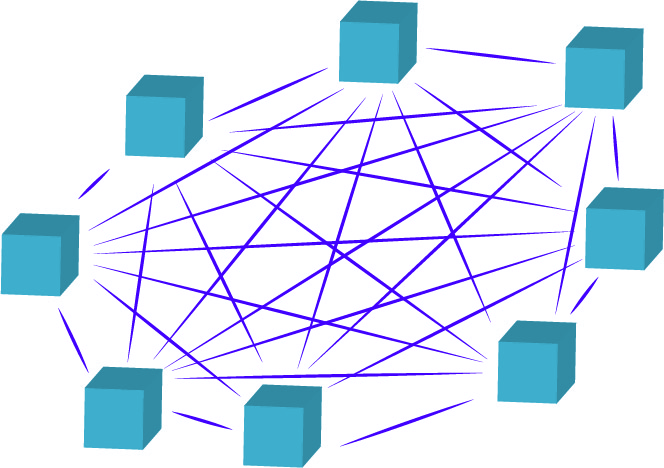
\includegraphics[width=\textwidth]{broadcasting}
  \caption{Broadcasting: The cubes represent peers and the lines represent connections between peers}
  \label{broadcastingfig}
\end{figure}

Broadcasting does not have this issue.
In broadcasting, every peer in the network is directly connected to each other, as depicted in figure \ref{broadcastingfig}.
Everyone personally takes care of their own advertising and there is no peer between origin and destination that could disrupt the communication.
The issue with broadcasting is that it scales rather poorly.
The increase of data over the network increases exponentially as the amount of users rises.
Because of this, using broadcasting in a large scale project is not advised.
However, broadcasting suffices for the first iteration.
Implementation is simple and it's easily replaced by a more complex system in later sprints.

\subsubsection{Protocol}
In this sprint, we also defined our application protocol.
For a detailed specification, see \ref{protocol}.
Although we have a lot of experience in using protocols and APIs, designing a new protocol is another matter entirely.
Our approach to designing the protocol was to keep it as simple as possible and make it easy to extend.
The goal is to make it easy to update the protocol, e.g, when there's a need to extend functionality.

\subsubsection{Broken Pipes}
Testing the socket connection showed a couple of issues.
Whenever a client would disconnect from a peer, the server that it was connected to reported a Broken Pipe error.
This however did not stop the server from running but it did add 2 empty string to the collection of received strings.
However if the server received an empty string that was sent intentionally, it ignores that message.
Therefor it would not hinder the communication if the Broken Pipe errors are suppressed, since the program will not change behaviour.
The empty strings that resulted from this error are now filtered out.

\subsubsection{Identifiers}
\label{sprint1:identifiers}
With the lack of a central authority confirming the identity of peers within the network, the users need an identifier of their own that distinguishes them from others.
This id needs to be unique to the peer and needs to be constructed as such that it cannot be imitated by someone else.
A regular username and password structure is not possible in a decentralised network since there is no entity that is trusted to store and confirm the passwords.


Simply using a username without a password is possible by broadcasting a request to receive all the usernames and allowing only nonexistent names to be used during creation.
While this creates a unique identifier for the user, it does not create a safety measure against impostors.
Anyone can declare that his username is Alice and can then validate transactions in the name of Alice, without the consent of the actual real Alice.

A solution to this problem lies in cryptography.
We need a way for users to prove that they are authentic.
Asymmetric encryption provides the solution.
The peers can use their public key as a unique identifier, since the chances of a SHA256 collision happening are incredibly low.
Users can now use the public key of the recipient of their message to force them to authenticate themselves.
As long as everyone stays the sole owner of their private key, no one but themselves will be able to respond correctly to the authentication request.
This enables a network where everyone can read every message, but can only answer to authentication requests when they are the original sender of the message.


\subsubsection{Cancelling}
\label{sprint1:cancelling}
We discussed how to cancel an ask or bid.
Our first proposal was to broadcast a special cancel message to all peers.
However, there are two major problems with this approach: authentication and flooding.


At the time of writing, a public key is used as identifier.
This means the same public key has to be used to send out the cancel message.
A single person should be able to create and dispose of public/private key pairs at will.
If, for whatever reason, the public/private key pair is lost, the ask/bid cannot be cancelled.


Another problem is the spoofing of these cancel messages.
Suppose a malicious third party sends out a cancel message.
Other users in the network cannot act on this message without authenticating the sender.
This would require three messages total.
Suppose Alice wants to send a cancel message to Bob.
The first is the cancel message from Alice to Bob.
The second is Bob asking Alice for verification, e.g.
by sending a random number encrypted by Alice's public key.
The third message would be Alice sending Bob the answer, proving she can unencrypt the random number.
This would quickly strain the network.


The solution to both of these problems is to not broadcast a cancel message at all.
If someone requests a trade to a cancelled ask/bid, it is replied to with a cancel message.
A timeout field is also added to every ask/bid.


Suppose Alice wants to cancel her ask/bid.
Internally, she will mark her ask/bid as cancelled.
If Bob requests a trade, Alice responds with a cancel message.
If Bob wants to authenticate Alice, he can piggyback a verification request with the trade message.
In the cancel message Alice responds with, she will also verify her identity with her private key.
This protocol only needs two messages, instead of three.
This exchange only happens between interested parties, instead of the entire network.
Lastly, this only occurs until the time of expiration.
\subsection{Sprint 2: Twisted and peer discovery}
In the second sprint, a networking library called Twisted is integrated into tsukiji. Instead of hardcoding peers, a peer discovery mechanism is introduced. Finally, a gossip protocol replaces the broadcasting protocol.

\subsubsection{Twisted}
\label{sprint2:twisted}
The networking protocol using raw sockets of sprint 1 showed how the idea of the implementation would work in practice.
What we need now is a stable and well-tested implementation to further our project into scaling and to prepare it for the real deal.
To save us the work required to produce such code, we chose to use a library instead.

Twisted is a open source library that offers many options for networking and communication. 
Their site describes it as an event-based framework for internet applications. Using this framework, rather than our self-made code had a couple of benefits:
\begin{itemize}
\item Twisted is well-tested.
\item Twisted is event-driven.
\item Twisted has an implementation of the UDP protocol.
\item Twisted is already implemented.
\end{itemize}
The current implementation of the broadcasting protocol of sprint 1 does not contain any tests so there is no guarantee that the code is bug-free and ready to be extended.
Twisted on the other hand has numerous test cases that cover many use-cases.
Because of this, a lot of time can be saved by trusting that the imported functions of Twisted will behave as promised instead of writing tests for our own implementation.

The current implementation uses a threaded approach to handling requests.
Threads are not maintained particularly well.
This is a enormous strain on the processor and the overall behaviour of the computer running the program.
Twisted gives a structure that requires a low amount of recourses when it is not handling data for sending or receiving messages with an event-driven engine.

Torrenting networks generally use UDP implementations to transport their data.
Keeping in line with this, it would be useful to have a similar way of handling communication in extensions of these programs.
Twisted provides options for both TCP and UDP.


All of the above issues could be made and added to the current TCP implementation made in the previous sprint.
This would however cost a lot of time that could be spent on trying to solve different issues that do not have such an easy outcome.

Given these advantages, Twisted seems like a great way to improve the current networking implementation and provide reliability and scalability.

\subsubsection{Peer discovery}
\label{sprint2:peerdiscovery}
One issue of having a decentralised system is that there is no central authority that can provide information about all the users and all the data. 
Because of this, when a peer is not yet part of the network, it has no knowledge of who to contact for more information about the network and all the peers connected to it. 
This problem of peer discovery has not yet been solved in a truly decentralised way. 
The current solution is to bootstrap a user by giving them a peerlist.
This peerlist contains a number of "super peers" that should always be online. 
The new peer then connects with one random super peer. 
This super peer sends a list of other peers back to the new peer.
Now the new peer knows about who is in the network.
From now on, the exchanging of peer lists does not necessarily have to occur with a super peer, but can also occur with other, regular peers.
With this implementation, the system is still mostly decentralised, but it still requires a number of super peers to be online to support the initial connection of a new user.

\subsubsection{Gossip}
\label{sprint2:gossip}
The implementation of sprint 1 used the broadcasting protocol to bring information of one peer to all the other peers.
This protocol is easy to implement but does not scale well. 
When the network grows larger, every peer has more recipients to contact and there are more peers sending messages all around.
To increase the scalability, a better protocol is required.
\begin{figure}[H]
  \centering
  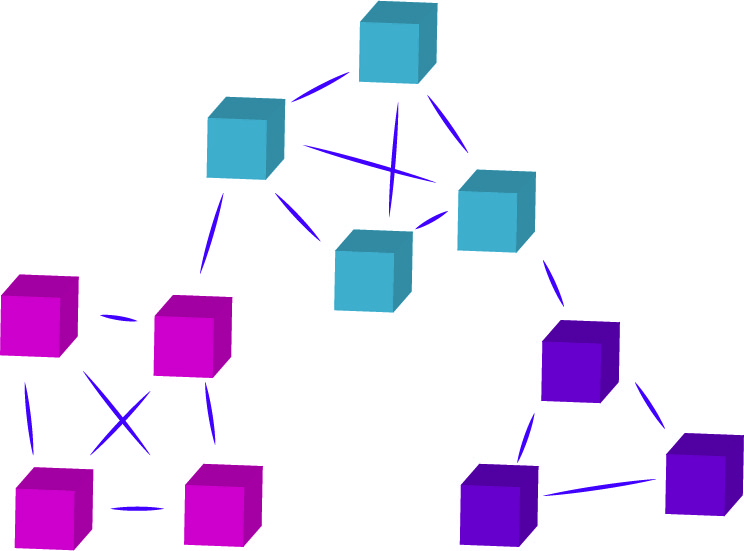
\includegraphics[width=\textwidth]{gossip}
  \caption{Gossip: The color of the cubes represent the groups of the peers and the lines represent connections between peers}
  \label{gossipfig}
\end{figure}
The peer discovery discussed in the previous section inherently creates a situation where subgroups of peers are created that know each other.
A peer can be in multiple groups and they provide the connection between groups.
The collection of groups connected to each other is called a clique.
This property of the network is exactly what an epidemic or gossip protocol uses.
In this type of protocol, a peer relays all the messages it receives to all peers in its group, which eventually spreads through the entire clique, as shown in figure \ref{gossipfig}.
Since the peers in a group have randomly chosen who sends them their peerlist, every peer should have a slightly different group of other peers that it knows.
Even in the case that every peer only encounters users within its own subgroup, the original master-peers can still act as a bridge between the groups.

Using the gossip protocol severely reduces network traffic compared to the broadcasting protocol.
The addition of a new user now only increases load of one group, rather than every peer in the network.
With the addition of many new peers, new groups will form to cut down the overall stress.
This protocol has proven itself to be scalable.
\subsection{Sprint 3: Testing at scale}
The theme of the third sprint is testing.
Testing is an important part of software development.
It gives the developers certainty over the quality of their program.
We felt like this sprint would be the perfect time to start testing.
It is better to start testing as early as possible.
We started relatively late compared to, for example, the Test Driven Development methodology, where tests are written even before the application logic is written.
However, it has allowed us to quickly iterate on Tsukiji in the early sprints.
At this stage, Tsukiji had reached a level of maturity where logic starts to become significantly more complex.
Tests give us assurance our program works correctly for the test cases we have defined.
There are two forms of testing focused on during this sprint: unit testing and scalibility testing.
Another form of testing that isn't focused on during this sprint is integration testing.
The purpose of integration testing is combine the components of a system and to test whether or not they produce the desired result.
However, at this point tsukiji is still sufficiently small that we believe producing such tests would yield little benefit.

\subsubsection{Unit testing}
Unit testing is the testing of small units of code, ideally the smallest block of code possible.
For our purposes, the smallest block of code is an individual function or class method.
Each unit should be tested in isolation, i.e. each test case is independent of each other.

\subsubsection{Scalibility testing}
The other form of testing focused on during this sprint is large scale testing.
The purpose of our large scale test is to test how functional the network remains with a large amount of peers.
\subsection{Sprint 4: Using real money}
With the implementation so far tested and polished, the time had come to implement our final feature. 
The last major challenge remaining at this point was linking the virtual marketplace to the real world.
So far users can trade their digital commodities for an amount of virtual currency.
The problem was that this currency had no actual value, since the only way of obtaining it was by trading it for reputation points.
So the marketplace at this point would consist out of people selling reputation points and others that do not have the means to acquire their own points, trying to buy them.
Sadly there would be no transactions made since no one had any virtual currency to make the first trade.
The solution to this problem is to allow users to use real money to either buy the virtual currency or use that money directly in the transaction.

\subsubsection{Usage of virtual currency}
Virtual currency is a great way to keep the identities of users hidden when making financial transactions. 
The problem this structure brings is that it requires a way to verify whether the digital money is actually real. 
When not using a central entity that governs the transactions, it becomes very difficult to tell where money came from and whether the balances of users are not tempered with.
There are of course solutions to this.

For example, you could implement a block-chain structure like BitCoin has made \cite{bitcoin}.
With this the whole user-base has to agree on a certain chain of transactions.
To achieve this, it is required to have every user communicate with every other user what transactions are made.
This way of regular broadcasting scales terribly and is the reason Tsukiji switched to a gossip model.

The solution for Tsukiji was to leave the idea of virtual currency completely. 
If users can use existing payment options, we no longer have to worry about security en legitimacy issues that payments bring.
The only thing that is required of Tsukiji is to link one peer to another peer and allow an easy way to perform the transaction.
The privacy issue is now brought back to the user. 
If they want to make anonymous transactions, they will have to create a separate account to make and receive transactions, that is not linked to their identity. 

\subsubsection{Online banking}
To use real money we required third party software to handle payments for us. 
After some research two options had our preference: iDeal and Paypal.
Sadly the iDeal API had a constraint that it only allowed users to give money to a business and not from person to person.
This would mean that every user has to create a business-account and have it approved by iDeal, just to make payments in Tsukiji.
As this is not deemed feasible, we chose to use Paypal instead.

The Paypal API offers many ways to create, send and verify transactions.
While poorly documented, there is a python integration that uses http calls with JSON objects to communicate with the Paypal servers.
The current implementation in Tsukiji creates a payment that has the amount (in euros) and the recipient pre-filled whenever a trade is made.
All the user has to do now, is fill in their login details on the Paypal page that opens automatically to authorise the transaction.
This way the user does not need to trust Tsukiji with their Paypal credentials and does not even need to know the address of the person they are about to pay.
This approach keeps Tsukiji decentralised as well, since the Paypal service is not part of the implementation of Tsukiji itself.

Tsukiji now has a way for users to pay eachother that is reliable but leaves itself unaccountable for any errors in transactions.
Users only have to trust Paypal for their transactions, which complies with the zero-trust ideology of a decentralised system.


% \section{Conclusion}
% \section{Discussion}

\bibliographystyle{plain}
\bibliography{refs}
\begin{appendices}
\newpage
\section{SIG feedback}

This appendix describes the feedback received from the Software Improvement Group (SIG) and how we processed the feedback.
On the 26th of May 2015, project code was sent to SIG for feedback.
Feedback on our code was received on the 29th of May.
After processing this feedback, a second code submission was sent on June 9th.
The second feedback response was received on June 17th.

\subsection{First feedback}

De code van het systeem scoort bijna vier sterren op ons onderhoudbaarheidsmodel, wat betekent dat de code bovengemiddeld onderhoudbaar is.
De hoogste score is niet behaald door een lagere score voor Component Balance en Unit Interfacing.


Wat opvalt bij het bekijken van de code is dat er geen duidelijke componenten-structuur zichtbaar is op het file-systeem, terwijl het er wel op lijkt dat sommige files bij elkaar horen (bijvoorbeeld de twee 'udp' files).
Dit maakt het voor een ontwikkelaar in eerste instantie lastiger om een algemeen beeld te krijgen van de functionaliteit die het systeem aanbied.
Wij raden aan om kritisch te overwegen om de code in verschillende (functionele) componenten op te delen om zo een eerste indruk te geven van de high-level structuur van het systeem.


Voor Unit Interfacing wordt er gekeken naar het percentage code in units met een bovengemiddeld aantal parameters.
Doorgaans duidt een bovengemiddeld aantal parameters op een gebrek aan abstractie.
Daarnaast leidt een groot aantal parameters nogal eens tot verwarring in het aanroepen van de methode en in de meeste gevallen ook tot langere en complexere methoden.
Binnen dit systeem wordt er op meerderee plaatsen een combinatie van 'price' en 'quantity' meegegeven, iets wat samen het concept 'bid' lijkt te vormen.
Ook zien we op meerdere plekken een 'host' / 'port' combinatie, deze vormen samen het concept 'peer'.
Om bij toekomstige aanpassingen duidelijker te maken wat er precies meegegeven moet worden aan deze methodes en om de code duidelijker te maken is het aan te raden een specifiek type te introduceren voor deze concepten.


Over het algemeen scoort de code bovengemiddeld, hopelijk lukt het om dit niveau te behouden tijdens de rest van de ontwikkelfase.
Als laatste nog de opmerking dat er geen (unit)test-code is gevonden in de code-upload.
Het is sterk aan te raden om in ieder geval voor de belangrijkste delen van de functionaliteit automatische tests gedefinieerd te hebben om ervoor te zorgen dat eventuele aanpassingen niet voor ongewenst gedrag zorgen.

\subsection{Response to feedback}
Three points of attention are given in the feedback: component balance, unit interfacing, and testing.

We agree on the points regarding component balance.
At the time, the code was split up into three main files: orderbook.py, crypto.py, and udpreceive.py.
While the first two files are fairly self-explanatory, udpreceive is fairly ambiguous.
There were also some extraneous components (e.g. udpsend) that were not core to the system, but possibly confusing to newcomers.
In response to this feedback, udpreceive.py was renamed to trader.py.
This more accurately describes what this file stands for.
If you invoke trader.py, you start up a new trader server.
However, we find it difficult to split the remaining parts up into more components.

The second point given talked about unit interfacing.
In this case, we believe SIG's feedback to be correct, but their solution undesirable.
It is true that many functions contain many arguments.
A lot of these shared common functionality, so we have abstracted these further into a main function.
However, SIG's solution is to introduce more classes.
In our project, these classes would be little more than packaging.
Rather than using classes, we use a lot of pure functions that return python dictionaries, and good variable names.
These can be seen as a replacement for classes.
There's a great talk from pycon 2012 called "Stop writing classes" \cite{noclassesvid}.
We believe the principles given in this talk to apply to our situation here.

The final piece of feedback given talked about testing.
We agree completely with this feedback and have since then implemented our own test suite.
The process of creating this test suite is described in section \ref{methodoloy:sprint3}.

\subsection{Second feedback}

In de tweede upload zien we dat zowel het codevolume als de score voor onderhoudbaarheid ongeveer gelijk zijn gebleven.

Bij Unit Interfacing zien we dat jullie een aantal methodes hebben aangepast, maar deze verbeteringen worden grotendeels weer ongedaan gemaakt door de introductie van nieuwe methodes met 3-4 parameters.
Dat lijkt niet zo veel, maar als je steeds het lijstje (price, quantity, timeout) tussen methodes moet doorgeven is dat een teken dat er iets in de abstractie niet helemaal lekker zit.

Bij Component Balance is onze eerste opmerking uit de analyse van de eerste upload nog steeds van kracht.

Jullie hebben onze aanbeveling om unit tests te gaan schrijven opgevolgd.
De hoeveelheid testcode die jullie sinds de eerste upload hebben geproduceerd is ook aanzienlijk, complimenten.
Op lange termijn zal dit zowel de onderhoudbaarheid als de stabiliteit van je systeem verbeteren.

Uit deze observaties kunnen we concluderen dat de aanbevelingen van de vorige evaluatie grotendeels zijn meegenomen in het ontwikkeltraject.

\subsection{Reponse to the second feedback}

The second round of feedback largely matches our response.
We have not adjusted unit interfacing because of the reasons explained previously.
We have not adjusted component balance in a major way.
We have added a lot of test code, which is acknowledged.
For the future course of this project, we will continue to keep a closer look at testing and component balance.
We do not believe unit interfacing poses a problem currently, but it is of course possible that it might in the future.
We will continue to monitor throughout the project's lifespan.
\newpage
\section{Original Project Description}
This project will create an electronic market place that is immune to shutdown by governments, immune to lawyer-based attacks or other real-world threats. The proof-of-concept marketplace will have no central server bottleneck, no central point of trust, full self-organization and unbounded scalability.\\
\\
To keep this project realistic, the focus will be on re-using existing code, support only Bitcoin-Euro trading, only use a single marketmaker, and offer no anonymity or DDoS protection. Bitcoin shows how vulnerable marketplaces are. Bitcoin was the first ever successful cybercurrency after decades of failures by  scientists, anarchists, fraudsters, and entrepreneurs. However, this first-generation technology suffers from an highly unstable exchange rate, low usage level and frequent large-scale thefts by hacking exchange platforms.

\end{appendices}


\end{document}

